\documentclass{article}
\title{Nechyba Ch.13 短期与长期的生产决策}
\author{Dawei Wang}
\date{\today}
\usepackage{ctex}
\usepackage{amsmath}
\usepackage{amssymb}
\usepackage{graphicx} %插入图片的宏包
\usepackage{float} %设置图片浮动位置的宏包
\usepackage{subfigure} %插入多图时用子图显示的宏包
\begin{document}
	\maketitle
用“经济环境”表示价格接受者在尽力做到最好时被当成既定的产出与要素的价格,继续通过“技术环境”表示如同生产边界总结的把要素转化为产出的技术过程。

\section{生产者行为随着条件变化的改变}、

\subsection{短期与长期不同类型的成本与花费}

沉没成本(sunk cost):不影响短期决策的经济成本,不管做什么都必须支付。

当所指为100\%的真实经济成本时,我们将其称为“成本”。但是如果支出包括沉没成本,则将其称为“支出”或“费用”。

由于在长期企业在调整要素束上有着更大的自由度,在短期要素的总支出永远不会比长期的生产成本低。但是由于短期中在固定要素上的固定支出不是一个真实的经济成本,从而认为企业的短期经济成本比长期经济成本高是不对的。

\begin{figure}[H] %H为当前位置,!htb为忽略美学标准,htbp为浮动图形
	\centering %图片居中
	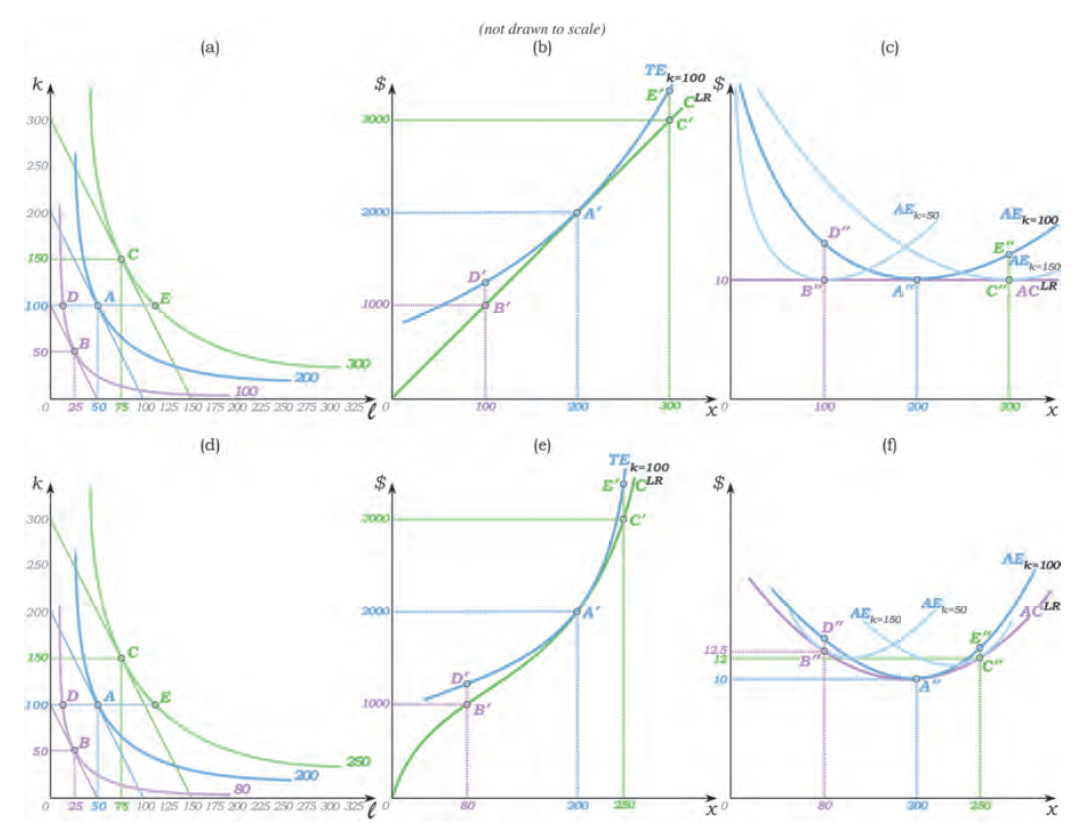
\includegraphics[width=1\textwidth]{13_1} %插入图片,[]中设置图片大小,{}中是图片文件名
	\caption{Short-Run Expenditure versus Long-Run Cost Curves} %最终文档中希望显示的图片标题
	\label{Fig.main2} %用于文内引用的标签
\end{figure}

在每种情形下,我都能断定生产的短期支出都会有比长期高,除了固定水平的资本恰好是长期中产量水平所对应的“正确的”水平。

\hspace*{\fill}

关闭与退出行业

一个企业愿意容忍多么低的产出价格并继续生产,以及价格下降到什么程度便不值得继续生产下去。答案将取决于我们分析的是短期的还是长期的问题而差别迥异。

因为一个企业由于在一定时期内被限制于固定的资本水平,实际上在短期不能完全消失。因为如果一个企业在短期中停止生产,我们将说它“关闭生产”,而如果它在长期中停止生产我们说它“退出行业”。

一个企业的“关闭价格”比“退出价格”低,这是因为在短期企业可以更容易地弥补它的经济成本,由于这些成本并不包括那些不管企业在做什么时都必须支付的固定资本的花费。换言之,尽管长期利润是负的,短期利润仍可能为正的,这意味着在短期中保持营业且在长期中不续约是经济理性的。

\begin{figure}[H] %H为当前位置,!htb为忽略美学标准,htbp为浮动图形
	\centering %图片居中
	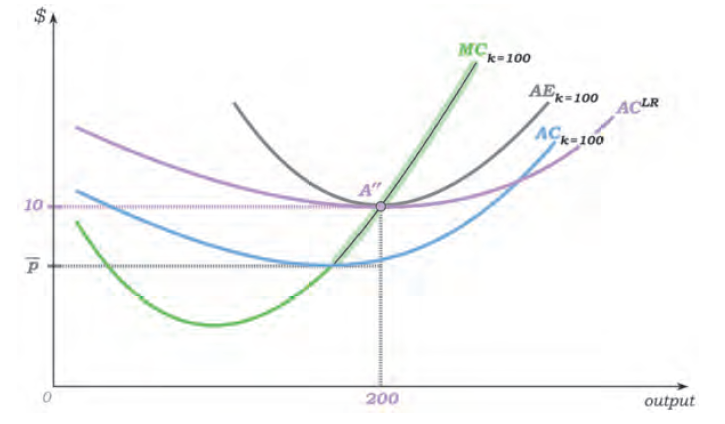
\includegraphics[width=1\textwidth]{13_2} %插入图片,[]中设置图片大小,{}中是图片文件名
	\caption{“Shut Down” versus “Exit” Price} %最终文档中希望显示的图片标题
	\label{Fig.main3} %用于文内引用的标签
\end{figure}

与固定要素相关的固定支出不是经济成本:它们不影响企业在短期中的经济决策。经济利润(economic profit)被定义为经济收益与经济成本的差额,当产出价格落在短期AC的最低点时经济利润恰好等于0。

\hspace*{\fill}

(长期)固定成本

在短期中,我们对长期中变得可变的固定要素的“成本”使用“固定支出”(FE)来表示。这样的成本称为(长期)可变成本,因为在长期中它们“随着产出变化”。

在长期中一个企业可能存在“固定的”(在它们不随着产出水平改变的意义上)但实际上代表可以避免的真实的经济成本的某种花费。称这样的成本为只有通过退出行业才能避免的固定的成本,或者简单地称为长期固定成本,因为它们可以通过退出行业来避免,所以是长期中真实的经济成本。如年许可证费。

\begin{figure}[H] %H为当前位置,!htb为忽略美学标准,htbp为浮动图形
	\centering %图片居中
	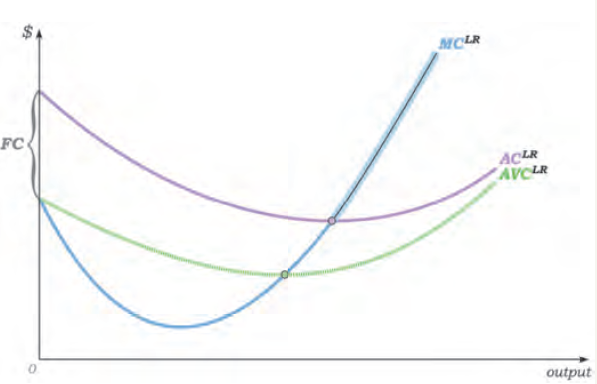
\includegraphics[width=1\textwidth]{13_3} %插入图片,[]中设置图片大小,{}中是图片文件名
	\caption{Long-Run Output Supply with Fixed Cost} %最终文档中希望显示的图片标题
	\label{Fig.main4} %用于文内引用的标签
\end{figure}

成本与支出类型概述

\begin{figure}[H] %H为当前位置,!htb为忽略美学标准,htbp为浮动图形
	\centering %图片居中
	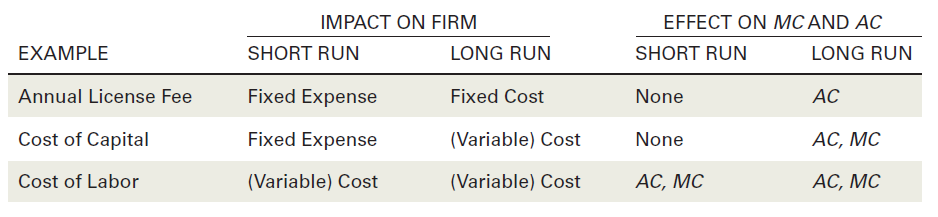
\includegraphics[width=1\textwidth]{13_4} %插入图片,[]中设置图片大小,{}中是图片文件名
	\caption{Examples of Costs and Expenses} %最终文档中希望显示的图片标题
	\label{Fig.main5} %用于文内引用的标签
\end{figure}

\begin{figure}[H] %H为当前位置,!htb为忽略美学标准,htbp为浮动图形
	\centering %图片居中
	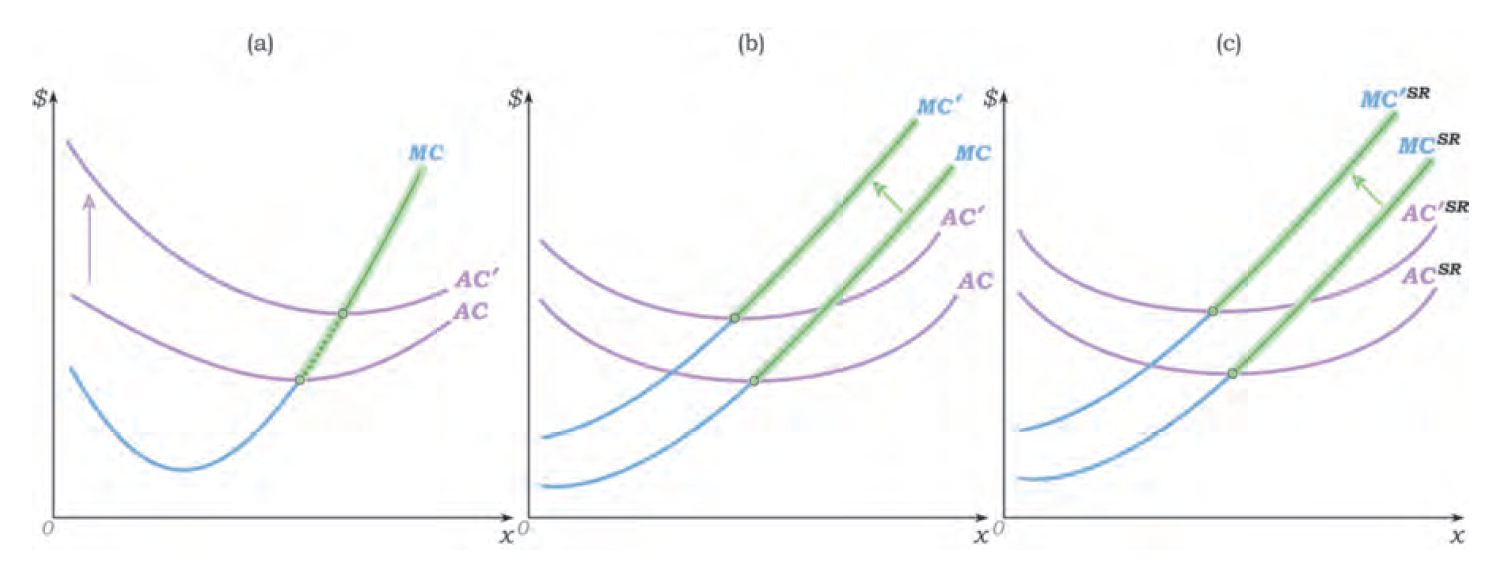
\includegraphics[width=1\textwidth]{13_5} %插入图片,[]中设置图片大小,{}中是图片文件名
	\caption{Three Types of Cost Changes} %最终文档中希望显示的图片标题
	\label{Fig.main6} %用于文内引用的标签
\end{figure}

其中,图(a)对应长期固定成本,图(b)对应资本成本,图(c)对应劳动成本。

长期AC曲线的最低点向左还是向右移动取决于潜在的技术,以及企业能替换资本与劳动的程度。

\subsection{短期和长期的产出供给}

\subsubsection{跨时的产出价格与供给}

假定一个生产者目前面对经济环境$ (w^A,r^A,p^A) $,并在ta的长期利润最大化的生产计划$ A=(l^A,k^A,x^A) $处生产。

市场处于长期均衡状态时的短期供给曲线(短期MC)与长期供给曲线(长期MC)都交于长期AC曲线最低点的经济直觉:

MC——边际成本,代表的是多生产一单位产品需要增加的成本,当市场处于长期均衡,$ MRP_l=MRP_k $,故此时在边际意义上纯增加l或者纯增加k(或任意比例的l与k混合)来获得额外的产品的成本是相同的。


\begin{figure}[H] %H为当前位置,!htb为忽略美学标准,htbp为浮动图形
	\centering %图片居中
	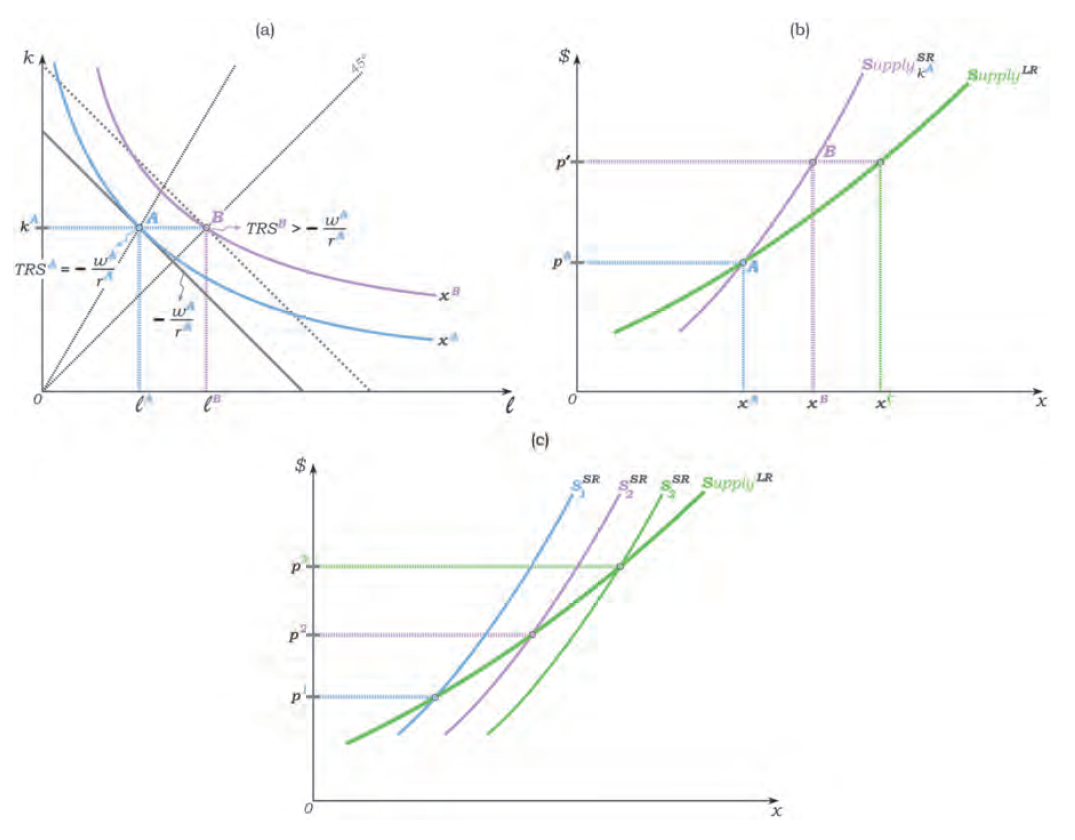
\includegraphics[width=1\textwidth]{13_6} %插入图片,[]中设置图片大小,{}中是图片文件名
	\caption{Short-Run versus Long-Run Supply Curves} %最终文档中希望显示的图片标题
	\label{Fig.main7} %用于文内引用的标签
\end{figure}

现假定产出价格上升到$ p' $,这将引起产出增加,但在短期中,生产者不能调整资本使其偏离目前的要素水平$ k^A $,此时:
\[
\frac{p'MP^B_l}{p'MP^B_k}<\frac{w^A}{r^A}
\]
同时,由于B点是当劳动完全可变时的短期最优,在B点的劳动边际产品收益一定等于工资$ w^A $,即$ p'MP^B_l=w^A $。从而$ p'MP^B_k>r_A $成立,换言之,在短期最优B点处,生产者能雇佣额外的资本,而其成本低于这些资本产生的额外收益。

当生产者在长期中能够调整资本时,ta会使用更多的资本,导致长期产出的增加超过短期产出的增加。从而长期供给曲线比短期供给曲线要平缓一些,表明生产者在长期比短期对产出价格的变化反应更大。

\subsubsection{长期供给与要素价格:生产中的替代效应}

产出价格的变化会引起生产者沿着供给曲线改变他们的生产行为,而要素价格的变化将会移动供给曲线,因为这样的变化导致了成本曲线的移动。由于随着要素相对价格的变化,生产者(至少在长期中)将会调整他们所使用的资本与劳动的比率来生产任意给定数量的产出,对于生产任意给定的产出水平的经济有效要素束也会随着要素价格的变化而变化。

\begin{figure}[H] %H为当前位置,!htb为忽略美学标准,htbp为浮动图形
	\centering %图片居中
	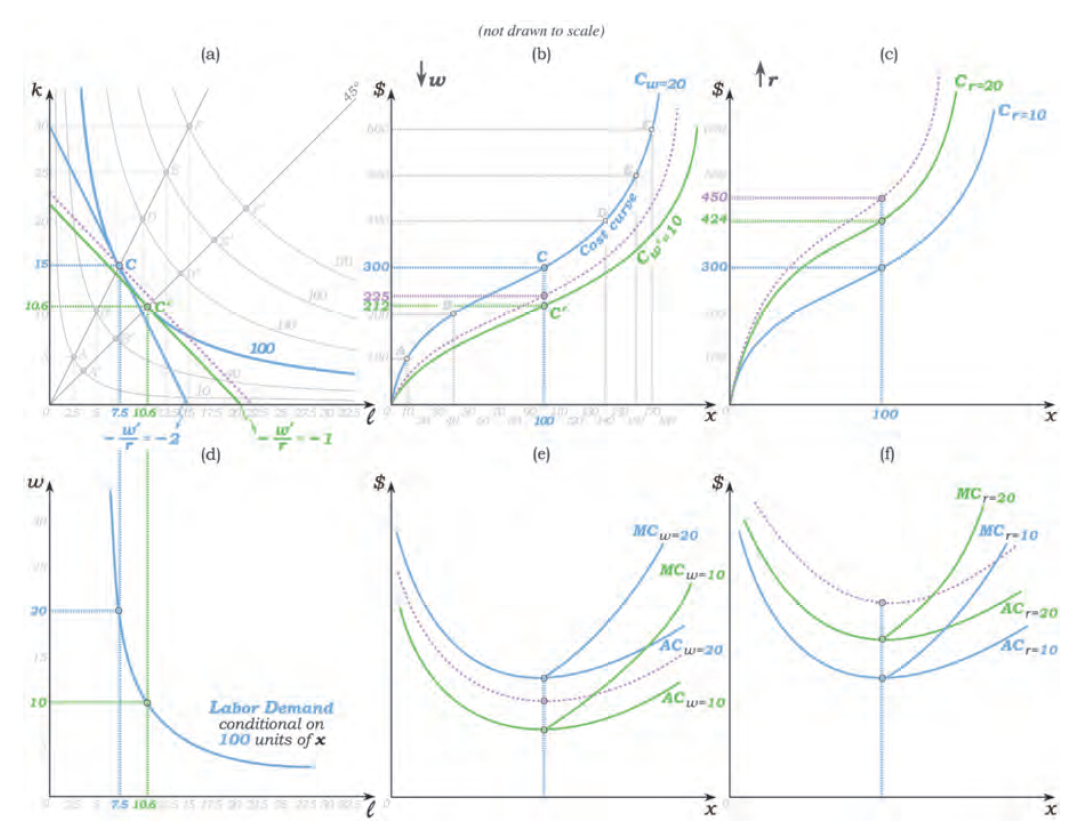
\includegraphics[width=1\textwidth]{13_7} %插入图片,[]中设置图片大小,{}中是图片文件名
	\caption{Costs and Input Substitution Effects} %最终文档中希望显示的图片标题
	\label{Fig.main8} %用于文内引用的标签
\end{figure}

替代效应总是使成本有降低的趋势。替代效应大小取决于生产过程中两个要素的替代程度。

一种对此进行表示的方式是条件要素需求曲线,其告诉我们在给定产出水平的条件下,生产者对要素的需求如何随着要素价格变化。条件要素需求曲线刻画了要素价格变化带来的纯替代效应。条件要素需求曲线取决于沿着生产一条等产量线的要素的替代性。

要素间的替代性越强,替代效应越大,条件要素需求曲线越平坦。反之反是。

当要素价格变化时,没有什么特别的原因使得长期AC曲线的最低点依然保持在相同的产出水平。依赖潜在的技术,最低点可能向左或者向右移动。然而对于固定的价格水平,供给的数量将会随着工资的下降而增加。

在短期中,当资本被固定时替代效应不会发生,短期供给曲线简单地显示为位于短期平均成本之上的MC曲线,可变要素地价格变化仅仅移动短期MC与短期AC。可以证明在长期中产出对要素价格地反映至少与短期一样大。

\subsection{要素需求与经济环境变化}

短期的劳动需求决策仅仅发生在当工资变化时边际收益产品曲线上。

短期产出价格p的变化会引起$ MRP_l $变化,而在长期,l和k都能被调整,因此长期劳动需求曲线将异于短期劳动需求曲线。

\begin{figure}[H] %H为当前位置,!htb为忽略美学标准,htbp为浮动图形
	\centering %图片居中
	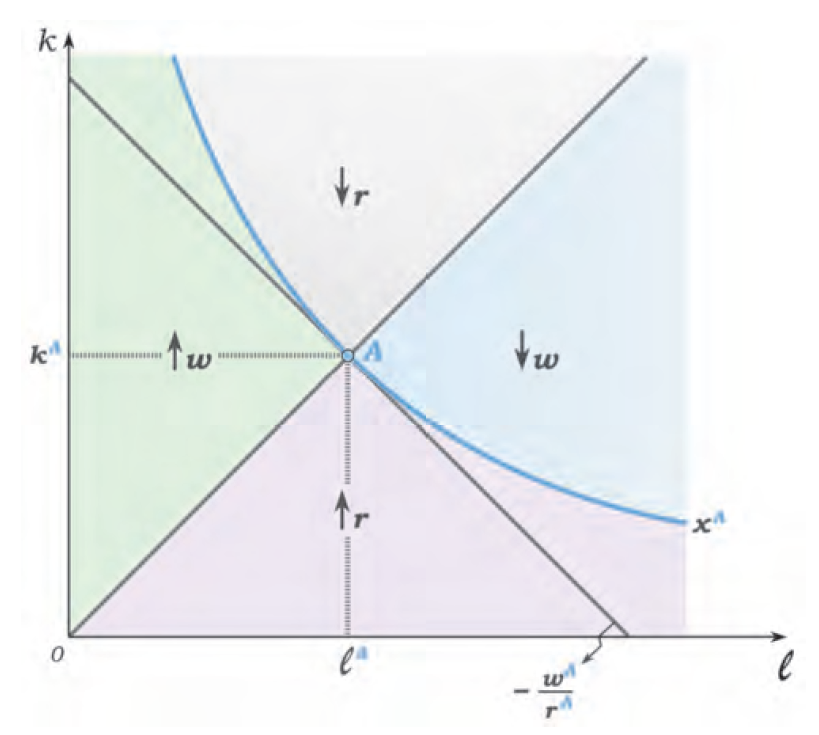
\includegraphics[width=1\textwidth]{13_8} %插入图片,[]中设置图片大小,{}中是图片文件名
	\caption{Changes in Input Prices and New Profit-Maximizing Input Bundles
		Combined} %最终文档中希望显示的图片标题
	\label{Fig.main9} %用于文内引用的标签
\end{figure}

\hspace*{\fill}

工资增加时的要素需求变化:
短期内,工资增加会导致劳动力需求减少,$ MP_l $增加。

若k与l之间存在较强替代性,则随着$ MP_l $增加,$ MP_k $也增加,这意味着$ pMP_k>r $,因此在长期我们将引进更多资本——解雇更多劳动力。

若k与l之间存在较强互补性,则随着$ MP_l $增加,劳动力减少,$ MP_k $减少,这意味着$ pMP_k<r $,因此在长期我们将减少资本——解雇更多劳动力。

综上:劳动需求对工资变化的长期反应总是大于短期反应。

\hspace*{\fill}

长期资本需求对工资变化的反应取决于资本与劳动的替代性。

\begin{figure}[H] %H为当前位置,!htb为忽略美学标准,htbp为浮动图形
	\centering %图片居中
	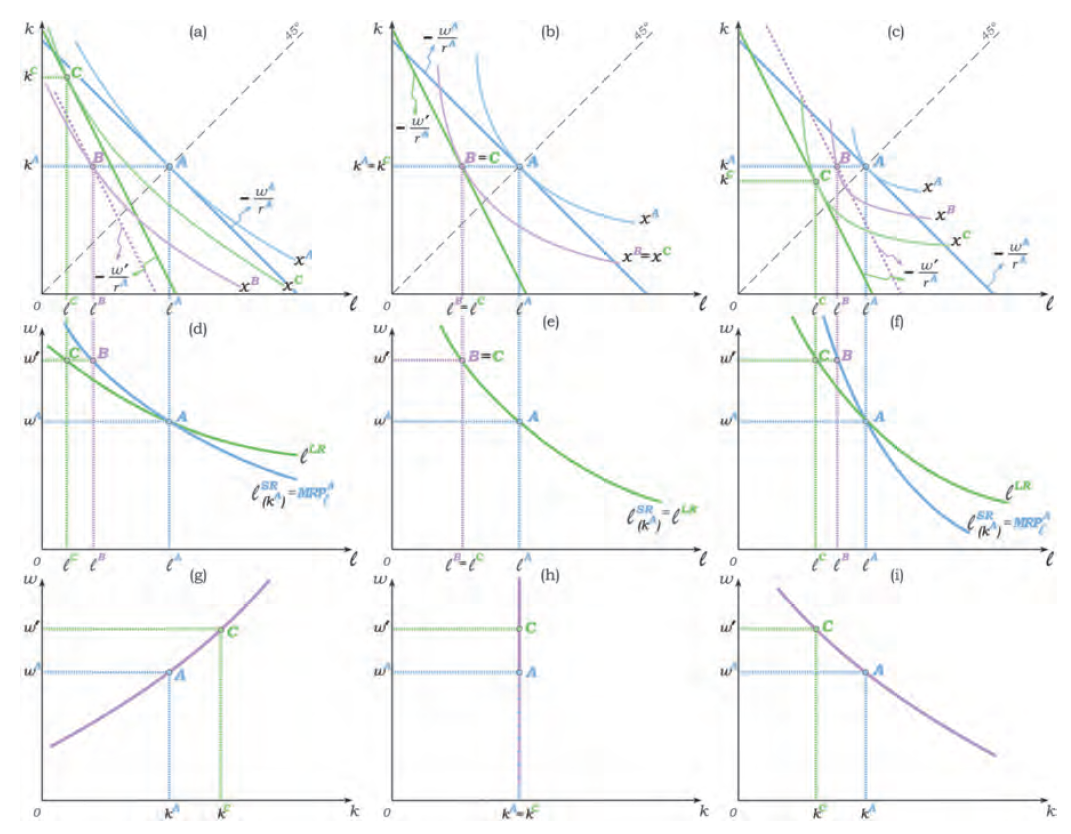
\includegraphics[width=1\textwidth]{13_9} %插入图片,[]中设置图片大小,{}中是图片文件名
	\caption{Short- and Long-Run Input Demand Responses when w Increases
		short} %最终文档中希望显示的图片标题
	\label{Fig.main10} %用于文内引用的标签
\end{figure}

\hspace*{\fill}

当r变化时劳动与资本的需求:

在短期资本成本的增加是一个沉没成本,从而不影响关于劳动、资本或短期产出的生产决策。

当r增加时,将导致一个新的位于包含A的等产量线的下方以及连接A与原点的射线右边的利润最大化的要素束。

\begin{figure}[H] %H为当前位置,!htb为忽略美学标准,htbp为浮动图形
	\centering %图片居中
	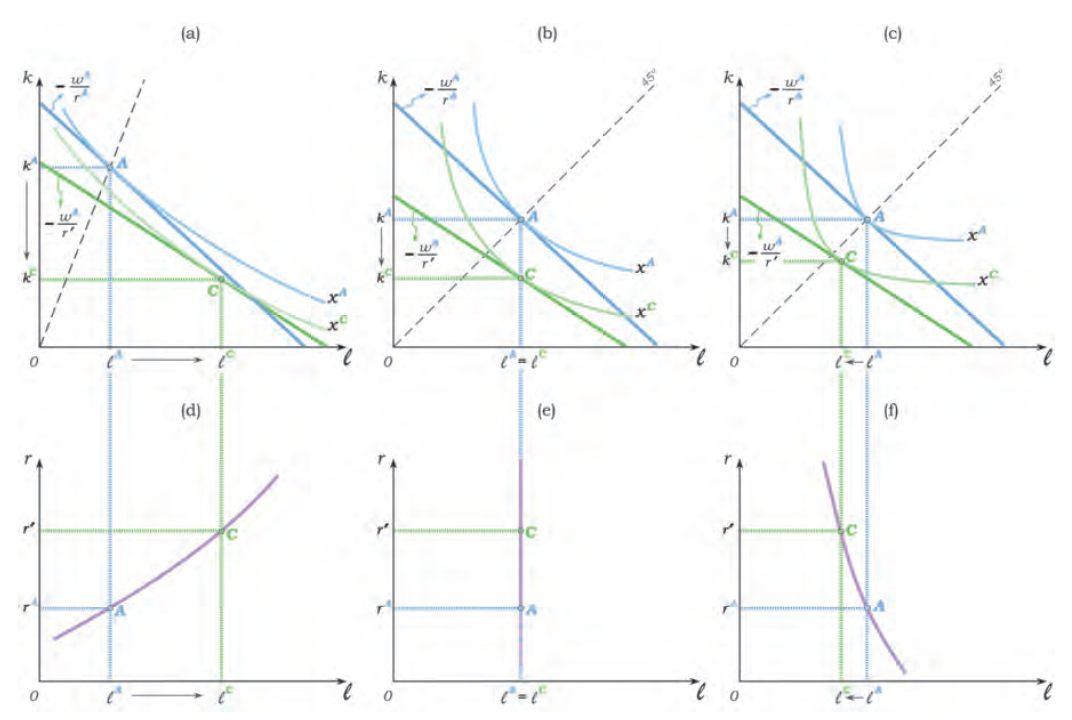
\includegraphics[width=1\textwidth]{13_10} %插入图片,[]中设置图片大小,{}中是图片文件名
	\caption{Long-Run Labor Demand Responses when r Increases} %最终文档中希望显示的图片标题
	\label{Fig.main11} %用于文内引用的标签
\end{figure}

当r增加时资本下降,可以断定长期资本需求曲线相对于r是向下倾斜,然而,当劳动和资本相对替代时r和l间的交叉价格关系可以向上倾斜,或者当劳动和资本在生产中相对互补时是向下倾斜。

\hspace*{\fill}

当P变化时劳动与资本的需求

在短期,资本可以是固定的,这意味着短期产出的增加完全源于额外被雇用的劳动。短期中劳动需求的增加是高些还是低些取决于在生产中资本与劳动的相对替代性。

\begin{figure}[H] %H为当前位置,!htb为忽略美学标准,htbp为浮动图形
	\centering %图片居中
	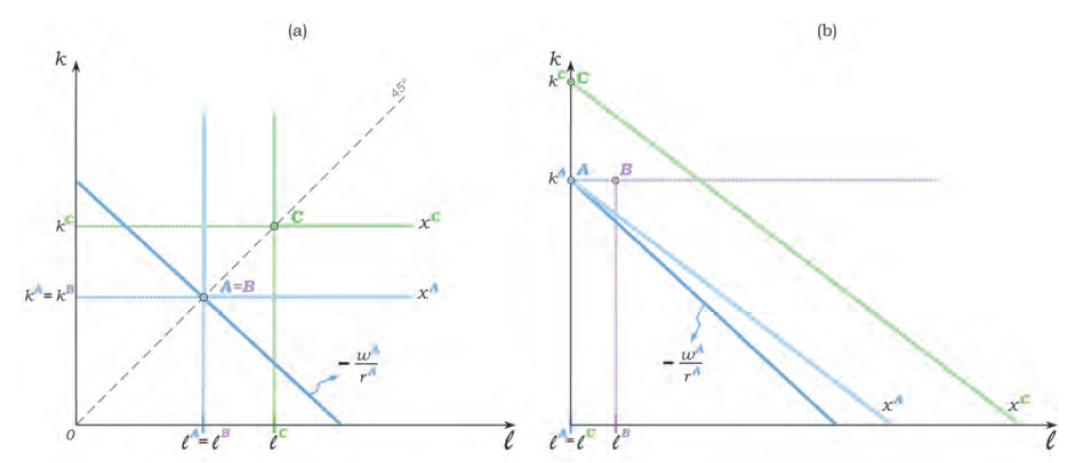
\includegraphics[width=1\textwidth]{13_11} %插入图片,[]中设置图片大小,{}中是图片文件名
	\caption{Input Demand Responses when p Increases} %最终文档中希望显示的图片标题
	\label{Fig.main12} %用于文内引用的标签
\end{figure}

产出价格变化所导致的劳动需求在短期中的反应可能比长期中的反应更大或更小,这取决于在生产中资本与劳动的替代程度。

\subsection{技术变化}

\begin{figure}[H] %H为当前位置,!htb为忽略美学标准,htbp为浮动图形
	\centering %图片居中
	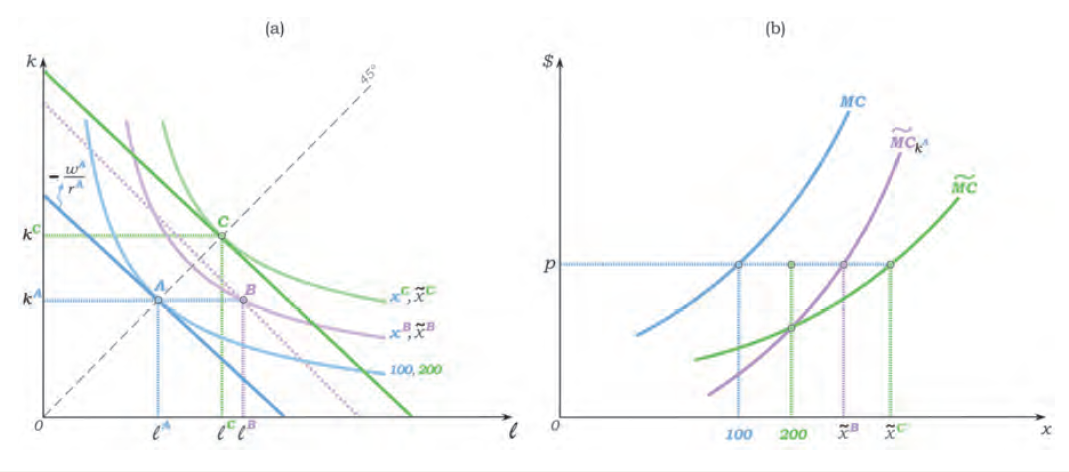
\includegraphics[width=1\textwidth]{13_12} %插入图片,[]中设置图片大小,{}中是图片文件名
	\caption{Technological Change that Raises MP/ and MPk Proportionately} %最终文档中希望显示的图片标题
	\label{Fig.main13} %用于文内引用的标签
\end{figure}

随着技术的变化,劳动和资本的边际产出在每个要素束处都更高,这意味着,如果生产者继续使用要素A,$ p\widetilde{MP}^A_l>w $且$ p\widetilde{MP}^A_k>r $,从而生产者将会在短期增加劳动知直到长期中可以调节资本。

\section{从短期到长期的数学转换}
给定生产函数(技术),利润最大化的生产计划(x,l,k)仅仅作为经济环境(P,W,r)的函数。

\subsection{花费与成本}
\subsubsection{短期支出与没有固定成本的长期成本}
假定$ k^A $是当要素价格为$ (w^A,r^A) $并且一个人要生产产出水平$ x^A $时使用的经济有效的资本水平。

短期中的劳动(条件)需求为:$ l_k^A(x) $

短期支出是:
\[
E_{k^A}(x,w^A,r^A)=w^Al_{k^A}(x)+r^Ak^A
\]
短期成本是:
\[
C_{k^A}(x,w^A)=w^Al_{k^A}(x)
\]

长期成本是通过求解如下成本最小化问题推导而得的:
\[
\min\limits_{l,k} wl+rk\enspace s.t.\enspace x=f(l,k)
\]

这些导致了条件要素需求l(x,w,r),k(x,w,r)与长期成本函数C(x,w,r)=wl(x,w,r)+rk(x,w,r)。当要素价格为$ (w^A,r^A) $时,长期成本是
\[
C(x,w^A,r^A)=w^Al(x,w^A,r^A)+r^Ak(x,w^A,r^A)
\]

$ x^A $对于$ k^A $是长期最优数量资本的产出水平等价于说$ k^A=k(x^A,w^A,r^A) $。如果企业在短期中开始有$ k^A $并决定生产$ x^A $,它可以把劳动设定到它的(长期)成本最小化水平,导致$ l_{k^A}(x^A)=l(x^A,w^A,r^A) $这意味着企业的短期支出等于长期成本。然而对于其他任意产出水平,$ k^A $通常不是长期最优水平,这意味着
\[
E_{k^A}(x,w^A,r^A)\ge C(x,w^A,r^A)
\]

\subsubsection{增加(长期)固定成本}

增加一个长期固定成本,则成本函数变为:
\[
\overline{C}(x,w,r)=C(x,w,r)+FC=wl(x,w,r)+rk(x,w,r)+FC
\]
\[
AC(x,w,r)=\frac{C(x,w,r)}{x}+\frac{FC}{x}=AVC(x,w,r)+\frac{FC}{x}
\]

由于FC/x随着x增加而下降,新的平均成本曲线收敛到平均可变成本。这意味着长期供给曲线并没有因为这样一个固定成本的增加而移动;它仅仅由于其起点随着AC曲线的上衣而向上移动,因而变得“短些”。

\subsection{产出供给与经济环境变化}

供给曲线为供给函数x(p,w,r)在保持要素价格(w,r)固定时的一个切片,并说明了产出供给如何随产出价格p的变化而变化。

Hotelling's Lemma 表明:
\[
\frac{\partial \pi(p,w,r)}{\partial p}=x(p,w,r)
\]

以及利润函数$ \pi(p,w,r) $关于p是凸的:
\[
\frac{\partial^2\pi(p,w,r)}{\partial p^2}\ge0
\]

得到
\[
\frac{x(p,w,r)}{p}\ge0
\]

因此产出供给函数在价格上是向上倾斜的(对短期生产函数也成立)。

\hspace*{\fill}

短期利润最大化的问题是:
\[
\max\limits_{x,l} px-wl\enspace s.t.\enspace x=f_{k^A}(l)
\]

解上述问题得到短期劳动需求函数$ l_{k^A}(p,w) $,并代回短期生产函数,我们得到短期产出供给函数$ x_{k^A}(p,w) $。此时劳动的MRP等于工资,但资本的MRP一般不等于租金率。

假定要素和产出价格恰好使得$ k^A $等于长期最优资本数量,此时短期利润减去在固定资本上的支出恰好等于长期利润;即$ \pi(p,w,r)=\pi_{k^A}(p,w)-rk^A $,如果$ k^A $不等于资本长期最优水平,短期利润减去$ rk^A $一定小于长期利润:
\[
\pi(p,w,r)\ge\pi_{k^A}(p,w)-rk^A
\]

定义:
\[
g(p)=\pi(p,w^A,r^A)=\pi(p,w,r)-\pi_{k^A}(p,w)+r^Ak^A
\]

g(p)在$ p^A $处达到最小值,这意味着g的二阶条件在$ p^A $处是正的。从而
\[
\frac{\partial^2g(p^A)}{\partial p^2}=\frac{\partial^2\pi(p^A,w^A,r^A)}{\partial p^2}-\frac{\partial^2\pi_{k^A}(p^A,w^A)}{\partial p^2}\ge0
\]
即
\[
\frac{\partial x(p^A,w^A,r^A)}{\partial p}\ge\frac{\partial x_{k^A}(p^A,w^A)}{\partial p}
\]

因此长期供给对产出供给的变化的反应要大于短期供给反应。

\hspace*{\fill}

生产中的替代效应

当要素价格下降时,生产成本也下降,既是因为目前成本最小化的要素束变得更便宜的直接效应,也因为较少密集使用相对较贵的要素的替代效应。

\subsection{要素需求与经济环境的变化}

要素需求曲线向下倾斜以及短期要素需求曲线比长期要素需求曲线更陡;

一种要素的需求与另一种要素的价格的“交叉价格”关系是不明确的并依赖于在生产中要素的相对替代性。

短期与长期劳动对产出价格变化的反应因要素的相对替代性而有区别。

根据Hotelling's Lemma:
\[
\frac{\partial \pi(p,w,r)}{\partial w}=-l(p,w,r)\enspace and\enspace \frac{\partial \pi(p,w,r)}{\partial r}=-k(p,w,r)
\]

根据利润函数对投入要素价格的凸性:
\[
\frac{\partial^2 \pi(p,w,r)}{\partial w^2}\ge0\enspace and\enspace \frac{\partial^2 \pi(p,w,r)}{\partial r^2}\ge0
\]

得到:
\[
\frac{\partial l(p,w,r)}{\partial w}\le0\enspace and\enspace \frac{\partial k(p,w,r)}{\partial r}\le0
\]


\end{document}